% Hinh: paper/paper1_qmi/figs_revision/fig10 (ban QMI, ve bang
% make_paper1_figures.py --qmi: o dKTA rong ruot, khong dem; cao hon ban TETC). Caption viet lai cho QMI: bo so BH
% 17/15/78 cu (hieu chinh hai lan), so BH dung nam o bang tab:multiplicity.
\begin{figure}[t]
  \centering
  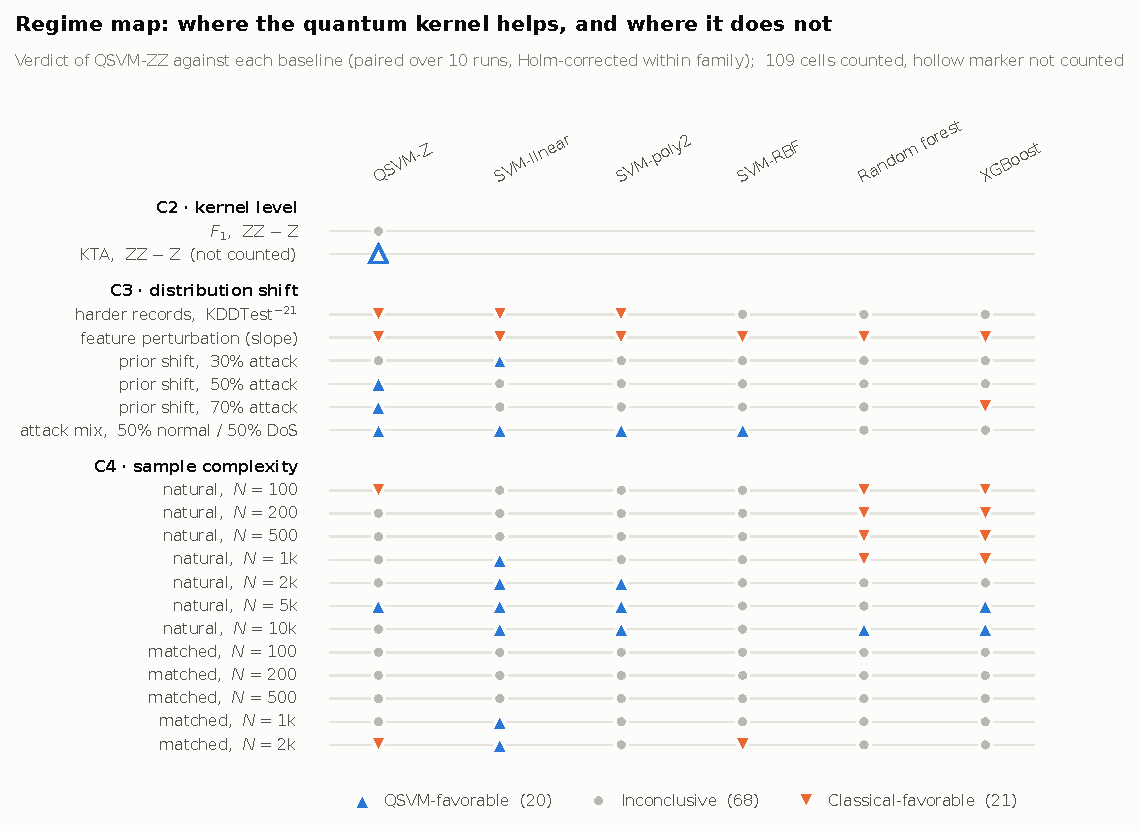
\includegraphics[width=\textwidth]{figs_revision/fig10_regime_map.pdf}
  \caption{Regime map of the controlled comparisons on NSL-KDD. Each marker is one
    paired comparison of \QSVM{} with one baseline over ten runs; colour and glyph both encode
    the verdict, Holm-adjusted within the baseline family. The \QSVM{}-\Zmap{} family has one
    member, so its cells are uncorrected. The hollow marker is the alignment check of
    Sec.~\ref{sec:res-ent}; it is shown but not counted, leaving $109$ counted cells. The seven rows of the training-set-size sweep
    under the natural prior ($42$ cells) form the single-protocol block of
    Sec.~\ref{sec:regime}; the other rows use the rare-enriched training pool
    (Table~\ref{tab:protocol}). Counts under other corrections are in
    Table~\ref{tab:multiplicity}.}
  \label{fig:regime-map}
\end{figure}
